\chapter{Force Sensors Overview}
\label{ch:overview}


This chapter is concerned about the basic functionality of force sensing resistor. A review of the technology is presented and typical characteristics are discussed. At the end the it is justified why using a FSR is used in extent of this thesis

\section{Previous Research}

Several techniques for the assessment of hand function have been devised over the past 70 years. Early methods focused on measuring dexterity rather than hand strength.\cite{nikonovas2004application} Used force sensors directly applied to the finger for hand positioning and force measurements. \cite{grosshauser2013finger} Applied a linear potentiometer directly on top of a violin fret to measure finger position.

\section{Force Sensing Resistors}


\section{FSR Technology Overview}
FSRs are polymer thick films (PTF) devices which exhibit a decrease in resistance when an external force is applied. The main composition can be broken into three main parts. A conducting and a resistive area which are separated by an adhesive spacer positioned at the verge of the FSR fig.\ref{fig:fsrcomposition}. The thickness of a FSR varies with desired design variables such as sensitivity and flexibility. At rest, the two polymer films do not touch each other, resulting in a non conductive state or high impedance. Once a force is exerted and contact between the two layers is established, the FSR becomes essentially a resistor.\newline
In contrast to load cells, FSR are not transducers. Neither are they strain gauges which rely on a change in resistance of a deformed resistor.\cite{giovanelli2016force}

\begin{figure}[ht]
    \centering
    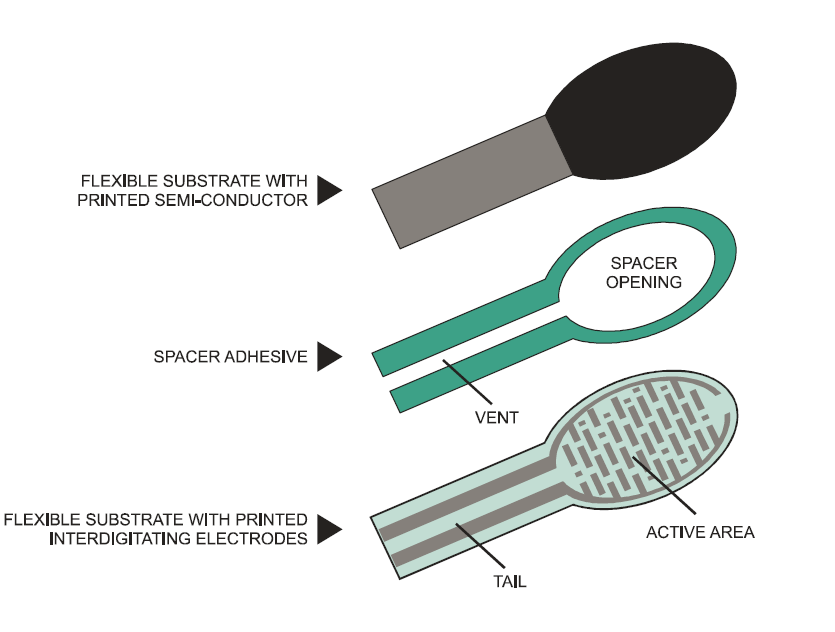
\includegraphics[width=0.75\textwidth]{images./fsr_parts.png}
    \caption[Individual Parts]{FSR individual parts. Source: \cite{interlinkelectronics}}
    \label{fig:fsrcomposition}
\end{figure}

\subsection{Sensor Setup}
\label{subsection:setup}
A typical senor setup is given in \ref{fig:setup}. The voltage drop across the load resistance is to be measured to lead back on the R\textsubscribt{F} value. In this configuration, the output voltage increases with increasing exerted force to the FSR as to be seen in fig \ref{fig:forcevalues}. If the resistors R\textsubscribt{FSR} and R\textsubscribt{L} were swapped, the output would decrease starting from supply voltage. The voltage across the load resistance can be described by a simple voltage divider:
\begin{equation}
    V_{out}=\frac{V_{dd}\cdot R_L}{R_L+R_{FSR}}
    \label{eq:divider}
\end{equation}
\begin{figure}[ht]
    \centering
    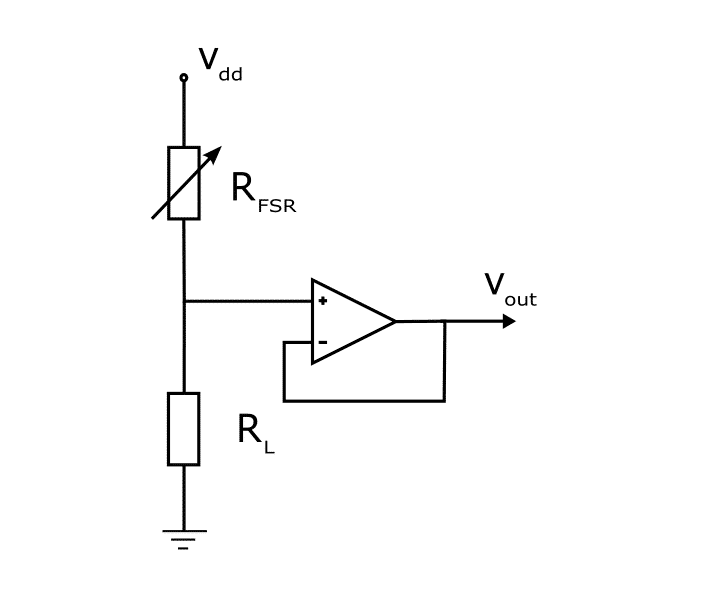
\includegraphics[width=0.75\textwidth]{images./FSR-1.png}
    \caption[FSR Setup]{Typical FSR Setup}
    \label{fig:setup}
\end{figure}




\section{FSR Performance Characteristics}
This section will be concerned about general characteristics of FSRs. Important to note at this point, that they are neither true force nor true pressure sensor, because of their area dependency on the measuring resistor. A true force sensor will always yield to the same signal for the same applied force regardless of position and area. 

\subsection{Force vs Resistance/ Conductance}
Fig \ref{fig:forcevalues} shows a typical characteristic of applied force versus measured voltage. For this characteristic, normed weights up to 1.6kg on a constant area of 3.5mm\textsuperscript{2} were used. It can bee seen that the force sensing resistor decreases in a non linear matter, at the high force end of the dynamic range, the response deviates from the power-law behavior, and eventually saturates to a point where increases in force yield little or no decrease in resistance. The saturation pressure of a typical FSR is in the order of 7 to 14 bar \cite{interlinkelectronics}.
\begin{figure}[ht]
    \centering
    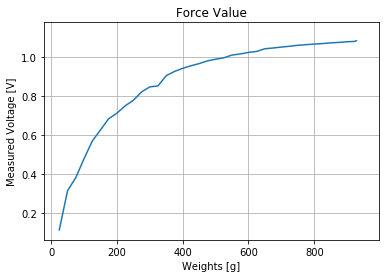
\includegraphics[width=0.75\textwidth]{images./Force.png}
    \caption[Force Characteristic]{Force Voltage Characteristic}
    \label{fig:forcevalues}
\end{figure}

\subsection{Accuracy}
\label{subsection:accuracy}
With proper mechanical arrangement, repeatability of an individual FSR is better than $\pm$ 2 \% over a specified force range. Variation between FSRs of a type is typically $\pm$ 15 \% \cite{yaniger1991force}. 




\section{Three Port Sensor}
In this thesis for the experiments a long FSR with an additional port on the resistor layer was used, see fig\ref{fig:scematic}. That additional port essentially turns the resistive layer into a linear potentiometer depending on force position.

which additionally allows position measurement. The schematic is presented in \ref{fig:FSR}.

\subsection{Sensor Schematic}
Figure \ref{fig:simplified} shows a simplified version of the given FSR. When pressure is applied on the surface the resistive layer at the bottom gets contact to the conductive layer hence creating a change in resistance. Resistor R\textsubscribt{F} is variable with contact size and force where R\textsubscribt{1} and R\textsubscribt{2} depend on position and area of the applied force. The corresponding schematic can be seen in fig. \ref{fig:schematic}



\begin{figure}[htp]
    \centering
    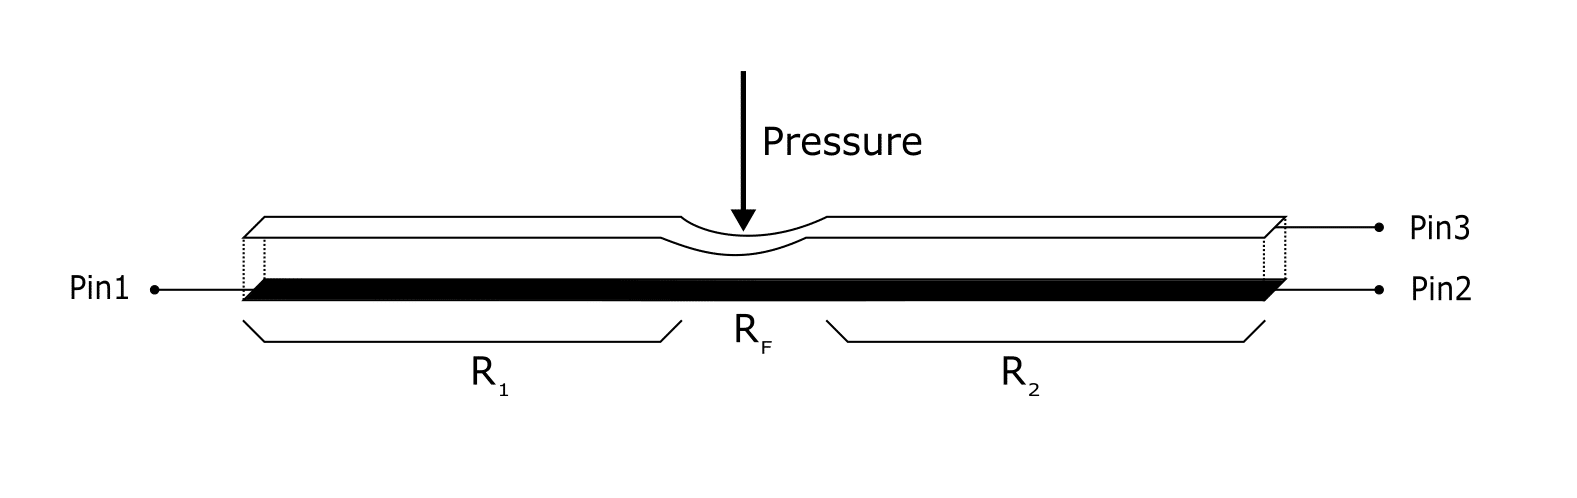
\includegraphics[width=\textwidth]{images./ForceSensor-1.png}
    \caption[FSR simplified]{Simplified Depcition}
    \label{fig:simplified}
\end{figure}  

\begin{figure}[htp]
    \centering
    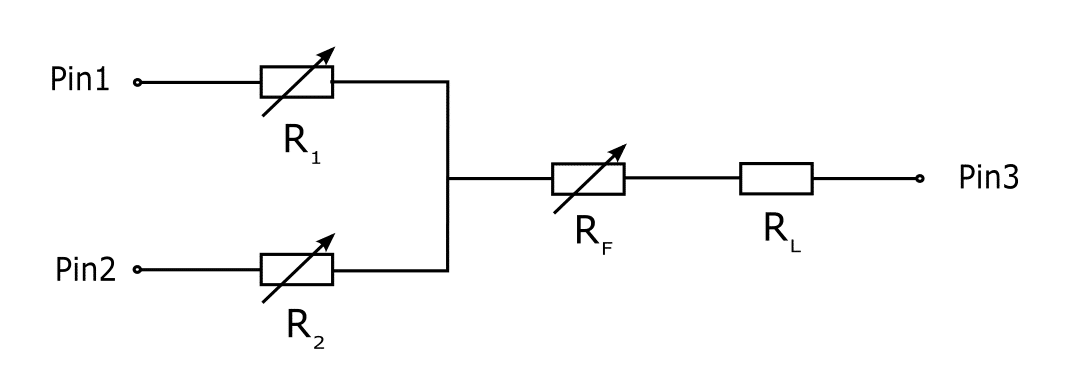
\includegraphics[width=\textwidth]{images./breakdown.png}
    \caption[FSR Schematic]{FSR Schematic}
    \label{fig:schematic}
\end{figure}  

\section{Operation Principle}
